\section{Riducibilità}
Vediamo un altro problema indecidibile
\paragraph{Il problema della fermata}
$HALT_{TM}=\{\langle M,w\rangle\mid M$ è una TM che si ferma su input $w\}$ 
Come possiamo dimostrare che $HALT_{TM}$ è indecidibile? 
Possiamo provare con la \g{diagonalizzazione} 
Sappiamo che $A_{TM}$ è indecidibile: \g{possiamo usare questo fatto per semplificare la dimostrazione?}

\paragraph{Riducibilità}
\begin{itemize}
	\item Una \g{riduzione} è un modo per trasformare un problema in un altro problema
	\item Una soluzione al secondo problema può essere usata per \g{risolvere il primo problema} 
	\item Se $A$ è riducibile a $B$, e $B$ è decidibile, allora $A$ è \g{decidibile} 
	\item Se $A$ è riducibile a $B$, e $A$ è decidibile, allora $A$ è \g{decidibile} 
\end{itemize}
\subsection{Dimostrazione per riduzione }
Queste dimostrazioni sono usate per dimostrare che un problema è indecidibile: 
\begin{enumerate}
	\item **Assumi** che $B$ sia decidibile
	\item **Riduci** $A$ al problema $B$ 
		\begin{itemize}
			\item costruisci una TM che usa $B$ per risolvere $A$ 
		\end{itemize}
	\item si $A$ è indecidibile, allora questa è una \g{contraddizione} 
	\item L'assunzione è sbagliata e $B$ è indecidibile
\end{enumerate}

\subsection{Il problema del vuoto}
$E_{TM} = \{\langle M\rangle\mid M$ è una TM tale che $L(M)=\varnothing\}$ 
\begin{itemize}
	\item La dimostrazione è per contraddizione e riduzione di $A_{TM}$ 
	\item Chiamiamo $R$ la TM che decide $E_{TM}$ 
	\item Useremo $R$ per costruire la TM $S$ che decide $A_{TM}$ 
\end{itemize}

\subsection{Stabilire se un linguaggio è regolare}
$REGULAR_{TM} = \{\langle M\rangle\mid M$ è una TM tale che $L(M)$ è regolare $\}$ 
\begin{itemize}
	\item La dimostrazione è per contraddizione e riduzione di $A_{TM}$ 
	\item Chiamiamo $R$ la TM che decide $REGULAR_{TM}$ 
	\item Useremo $R$ per costruire la TM $S$ che decide $A_{TM}$ 
	\item Capire come possiamo usare $R$ per implementare $S$ è meno ovvio di prima 
\end{itemize}

\subsection{Il problema dell'equivalenza}
$EQ_{TM} = \{\langle M_1,M_2\mid M_1, M_2$ TM tali che $L(M_1)=L(M_2)\}$ 
\begin{itemize}
	\item La dimostrazione è per contraddizione e riduzione di $E_{TM}$ (problema del vuoto)
	\item Chiamiamo $R$ la TM che decide $EQ_{TM}$ 
	\item Useremo $R$ per costruire la TM $S$ che decide $E_{TM}$ 
\end{itemize}

\subsection{Riducibilità mediante funzione}
Trasforma istanze del problema $A$ in istanze del problema $B$ mediante una \g{funzione calcolabile} 
\begin{itemize}
	\item Chiarisce e formalizza la riducibilità
		\paragraph{Definizione}
		$f:\Sigma^*\rightarrow\Sigma^*$ è una \g{funzione calcolabile} se esiste una TM $M$ che su input $w$, termina la computazione avendo solo $f(w)$ sul nastro
	\item Le operazioni aritmetiche sugli interi sono funzioni calcolabili
	\item Le trasformazioni di macchine di Turing possono essere funzioni calcolabili
\end{itemize}

Un linguaggio $A$ è \g{riducibile mediante funzione} al linguaggio $B$ $(A\leq_m B)$, se esiste una \g{funzione calcolabile} $f:\Sigma^*\rightarrow\Sigma^*$ tale che 
Per ogni $w:w\in A$ se e solo se $f(w)\in B$ \\
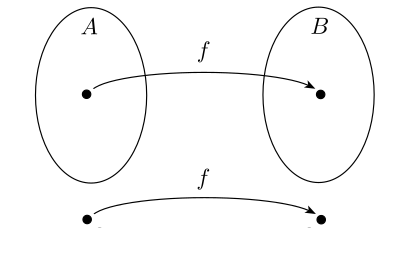
\includegraphics[scale=0.5]{img/funzione_riduzione.png}\\
$f$ è la **riduzione** da $A$ a $B$ 

Se esiste una \g{riduzione} da $A$ e $B$, possiamo risolvere $A$ usando una soluzione per $B$: \\
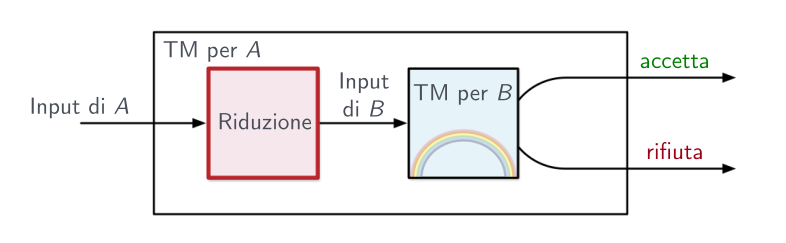
\includegraphics[scale=0.5]{img/schema_riducibilita.png}
\subsection{Proprietà delle riduzioni}
\paragraph{Teorema}
Se $A\leq_m B$ e $B$ è ???, allora $A$  è ??? 
\paragraph{Teorema}
Se $A\leq_m B$ e $A$ è  allora $B$ è ??? 

\subsection{Il problema della fermata(2)}
$HALT_{TM}=\{\langle M,w\rangle\mid M$ è una TM che si ferma su input $w\}$ 
\begin{itemize}
	\item Possiamo dimostrare che $A_{TM}\leq_m HALT_{TM}$ ? 
	\item Qual è l'input della funzione di riduzione? 
	\item Qual è l'output? 
	\item Quali proprietà devono rispettare? 
\end{itemize}
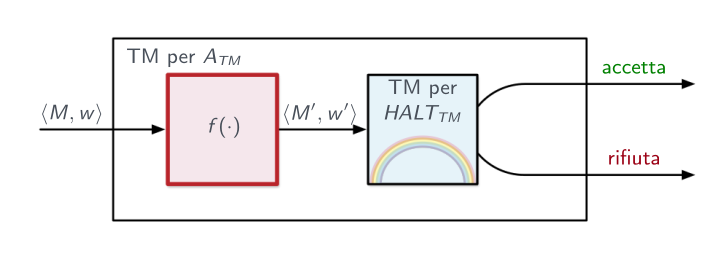
\includegraphics[scale=0.5]{img/schema_halt.png}\\
$M$ accetta $w$ se e solo se $M'$ si ferma su $w'$ 
\subsection{Il problema dell'equivalenza(2)}
$$EQ_{TM}=\{\langle M_1, M_2\rangle\mid L(M_1)=L(M_2)\}$$
\begin{itemize}
	\item Possiamo dimostrare che $E_{TM}\leq_m EQ_{TM}$ ?
	\item Qual è l'input della funzione di riduzione? 
	\item Qual è l'output? 
	\item Quali proprietà devono rispettare? 
\end{itemize}
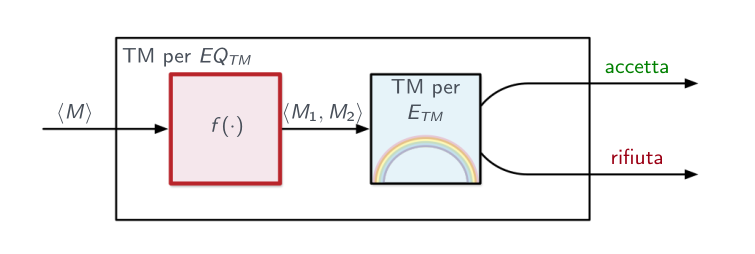
\includegraphics[scale=0.5]{img/schema_eq_tm.png}
$L(M)=\varnothing$ se e solo se $L(M_1)=L(M_2)$ 

\subsection{Il problema del vuoto(2)}
$E_{TM}=\{\langle M\rangle\mid M$ è una TM tale che $L(M)=\varnothing\}$ 
\begin{itemize}
	\item Possiamo dimostrare che $A_{TM}\leq_m E_{TM}$ ?
	\item Qual è l'input della funzione di riduzione? 
	\item Qual è l'output? 
	\item Quali proprietà devono rispettare? 
\end{itemize}
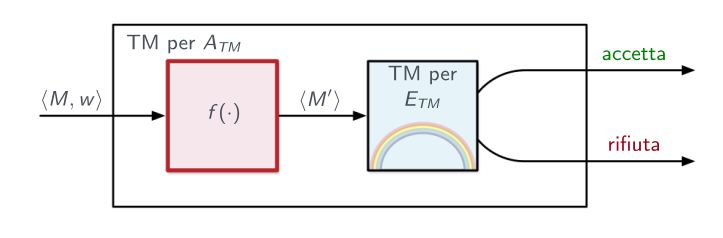
\includegraphics[scale=0.5]{img/schema_atm_etm.png}
$M$ accetta $w$ se e solo se $L(M')=\varnothing$ 
\begin{center}
	{\Large STOP!!!}
\end{center}
\g{Non sappiamo come ridurre il problema dell'accettazione al problema del vuoto!}
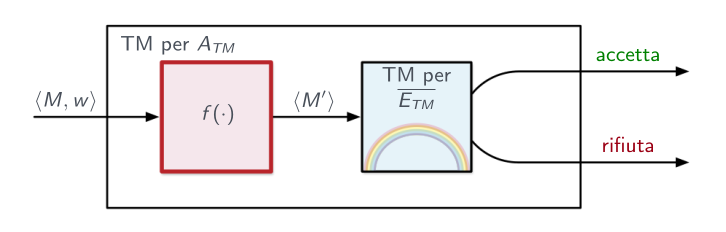
\includegraphics[scale=0.5]{img/schema_atm_etm_2.png}
$M$ accetta $w$ se e solo se $L(M') \neq \varnothing$ 
\paragraph{Proprietà delle riduzioni (2)}
\paragraph{Teorema}
Se $A\leq_m B$ e $B$ è ???, allora $A$  è ??? 
\paragraph{Teorema}
Se $A\leq_m B$ e $A$ è ???  allora $B$ è ??? 
